\title{eiPack: R $\times$ C Ecological
Inference and Higher-Dimension Data Management}
\author{by Olivia Lau, Ryan T. Moore, and Michael Kellermann}

\definecolor{DarkRed2}{rgb}{0.6,0,0.08}
\newcommand{\indep}{{\;\bot\!\!\!\!\!\!\bot\;}}

\maketitle

\section*{Introduction}

\dfn{Ecological inference} (\acronym{ei}) models allow researchers to infer
individual-level behavior from aggregate data when individual-level
data is unavailable.  Table 1 shows a typical unit of ecological
analysis: a contingency table with observed row and column marginals
and unobserved interior cells.
\begin{center}
\begin{tabular}{l|cccc|c}
	& $\rm{col}_1$ & $\rm{col}_2$ & $\ldots$ & $\rm{col}_C$ & \\
\hline
$\rm{row}_1\quad$	& \color{DarkRed2}{$\;\; N_{11i}\;\;$} & \color{DarkRed2}{$\;\; N_{12i}\;\;$} & $\ldots$ & \color{DarkRed2}{$\;\; N_{1Ci}\;\;$} & $\quad N_{1\cdot i}$ \\
$\rm{row}_2\quad$ 	& \color{DarkRed2}{$N_{21i}$} &
\color{DarkRed2}{$N_{22i}$} &  $\ldots$ &
\color{DarkRed2}{$N_{2Ci}$} & $\quad N_{2\cdot i}$ \\ 
 $\ldots$ & $\ldots$ & $\ldots$ & & $\ldots$ & $\ldots$ \\
$\rm{row}_R\quad$	& \color{DarkRed2}{$N_{R1i}$} & \color{DarkRed2}{$N_{R2i}$} & $\ldots$ &
\color{DarkRed2}{$N_{RCi}$} & $\quad N_{R\cdot i}$ \\ 
\hline
	& $N_{\cdot 1i}$ & $N_{\cdot 2i}$ &  $\ldots$ & $N_{\cdot Ci}$ & $\quad
N_i$\\
\multicolumn{5}{l}{}
\end{tabular} 

Table 1: A typical $R \times C$ unit in ecological inference;
{\color{DarkRed2}red} quantities are typically unobserved.
\end{center}

In ecological inference, challenges arise because information is lost
when aggregating across individuals, a problem that cannot be solved
by collecting more aggregate-level data.  Thus, \acronym{ei} models
are unusually sensitive to modeling assumptions. Testing these
assumptions is difficult without access to individual-level data, and
recent years have witnessed a lively discussion of the relative merits
of various models \citep{Wakefield04}.

Nevertheless, there are many applied problems in which ecological
inferences are necessary, either because individual-level data is
unavailable or because the aggregate-level data is considered more
authoritative.  The latter is true in the voting rights
context in the United States, where federal courts often base 
decisions on evidence derived from one or more \acronym{EI} models
\citep{Cho01}.  While packages such as \pkg{MCMCpack}
\citep{MartinQuinn06} and \pkg{eco} \citep{eco}, provide tools for $2 \times 2$ inference, this is
insufficient in many applications. In \pkg{eiPack}, we implement
three existing methods for the general case in which the ecological units are $R \times C$ tables.



\section*{Methods and Data in \pkg{eiPack}}

The methods currently implemented in \pkg{eiPack} are the method of
bounds \citep{DunDav53}, ecological regression \citep{Goodman53}, and
the Multinomial-Dirichlet model \citep{RosJiaKin01}.

The functions that implement these models share
several attributes.  The ecological tables are defined using a
common formula of the form \code{cbind(col1, ..., colC)} $\sim$
\code{cbind(row1, ...,rowR)}.  The row and column marginals can be
expressed as either proportions or counts.  Auxiliary functions
renormalize the results for some subset of columns taken from the
original ecological table, and appropriate \code{print},
\code{summary}, and \code{plot} functions conveniently summarize
the model output.

In the following section, we demonstrate the features of
\pkg{eiPack} using the (included) \code{senc} dataset, which
contains individual-level party affiliation data for Black, White, and
Native American voters in 8 counties in southeastern North Carolina.
These counties include 212 precincts, which form the ecological units
in this dataset.  Because the data are observed at the individual
level, the interior cell counts are known, allowing us to benchmark
the estimates generated by each method.

\subsection*{Method of Bounds}

The method of bounds \citep{DunDav53} uses the observed row and column
marginals to calculate upper and lower bounds for functions of the
interior cells of each ecological unit.  The method of bounds is not a
statistical procedure in the traditional sense; the bounds implied by
the row and column marginals are deterministic and there is no
probabilistic model for the data-generating process.

As implemented in \pkg{eiPack}, the method of bounds allows the user
to calculate for a specified column $k' \in k = \{1, \dots, C\}$ the deterministic bounds on the proportion of
individuals in each row who belong in that column.  For each
unit being considered, let $j$ be the row of interest, $k$ index
columns, $k'$ be the column of interest, $k''$ be the set of other
columns considered, and $\tilde{k}$ be the set of columns excluded.
For example, if we want the bounds on the proportion of Native
American two-party registrants who are Democrats, $j$ is Native
American, $k'$ is Democrat, $k''$ is Republican, and $\tilde{k}$ is No
Party.  The unit-level quantity of interest is

\begin{displaymath}
\frac{N_{jk'i}}{N_{jk'i} + \sum_{k \in k''} N_{jki}}
\end{displaymath}

\noindent The lower and upper bounds on this quantity given by the
observed marginals are, respectively:

\begin{displaymath}
\frac{\max(0, N_{ji} - \sum_{k \neq k'} N_{ki})}{\max(0, N_{ji} - \sum_{k \neq
k'} N_{ki}) + \min(N_{ji}, \sum_{k \in k''} N_{ki})}
\end{displaymath}

\noindent and

\begin{displaymath}
\frac{\min(N_{ji}, N_{k'i})}{\min(N_{ji}, N_{k'i}) + \max(0, N_{ji} - N_{k'i} - \sum_{k \in \tilde{k}} N_{ki})}
\end{displaymath}

The intervals generated by the method of bounds can be analyzed in a
variety of ways.  \citet{Grofman00} suggests calculating the
intersection of the unit-level bounds.  If this intersection (calculated by \pkg{eiPack}) is non-empty, it represents the range of values
that are consistent with the observed marginals in each of the
ecological units.  

Researchers and practitioners may also choose to restrict their
attention to units in which one group dominates, since the
bounds will typically be more informative in those units.  \pkg{eiPack}
allows users to set row thresholds to conduct this
\dfn{extreme case analysis} (known as \dfn{homogeneous
precinct analysis} in the voting context).
For example, suppose the user is interested in the proportion of
two-party White registrants registered as Democrats in precincts that
are at least 90\% White.  \pkg{eiPack} calculates the desired bounds:
\begin{smallexample}
> out <- bounds(cbind(dem, rep, non) ~ cbind(black,
+   white, natam), data = senc, rows = "white", 
+   column = "dem", excluded = "non",
+   threshold = 0.9, total = NULL)
\end{smallexample} %$
These calculated bounds can then be represented graphically.  Segments
cover the range of possible values (the true value for each precinct
is the red dot, not included in the standard bounds plot).  In this
example, the intersection of the precinct-level bounds is empty.
\begin{smallexample}
> plot(out, row = "white", column = "dem")
# add true values to plot
> idx <- as.numeric(rownames(out$bounds$white.dem))
> truth <- senc$whdem[idx]/(senc$white[idx]
+   -senc$non[idx])
> plot((1:length(idx)) / (length(idx) + 1), truth)
\end{smallexample}
\begin{figure}[h!]
\begin{center}
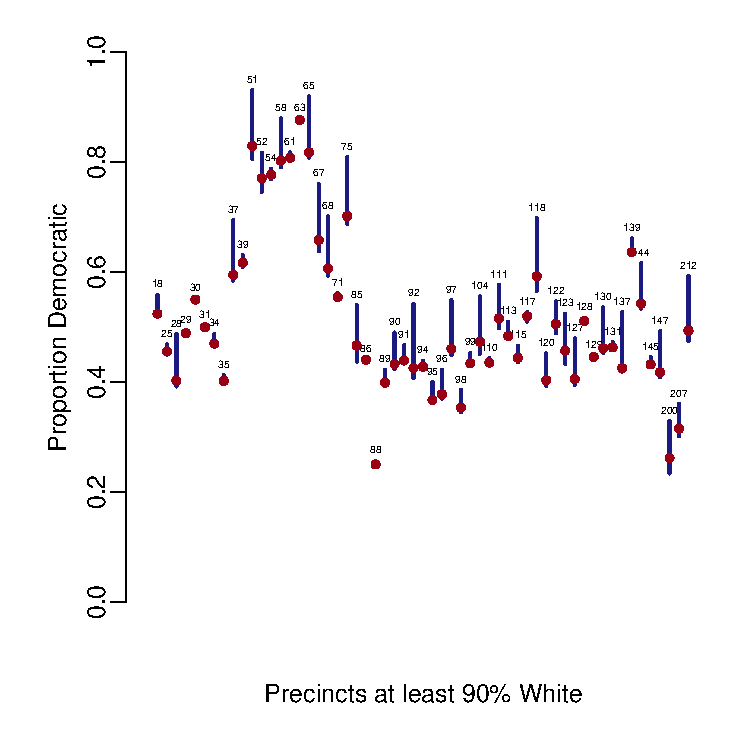
\includegraphics[height=3.2in]{white.pdf}
\end{center}
\caption{A plot of deterministic bounds.}
\label{f:mob} 
\end{figure}
%$
\subsection*{Ecological Regression}

In ecological regression \citep{Goodman53}, observed row and column
marginals are expressed as proportions and each column is regressed
separately on the row proportions, thus performing $C$ regressions.  
Regression coefficients then estimate the population internal cell
proportions.  For a given unit $i$, define

\begin{itemize}
\item $X_{ri}$, the proportion of individuals in row $r$,
\item $T_{ci}$, the proportion of individuals in column $c$, and
\item $\beta_{rci}$, the proportion of row $r$ individuals in column
$c$
\end{itemize}

\noindent The following identities hold:
\begin{displaymath}
T_{ci} \; = \; \sum_{r=1}^R \beta_{rci} X_{ri} \quad \textrm{and} \quad \sum_{c=1}^{C} \beta_{rci}  \; = \; 1    
\end{displaymath}
\noindent  Defining the population cell fractions $\beta_{rc}$ such that
$\sum_{c=1}^C \beta_{rc} = 1$ for every $r$, ecological regression assumes that
$\beta_{rc} = \beta_{rci}$ for all $i$, and estimates the regression
equations $T_{ci} = \beta_{rc} X_{ri} + \epsilon_{ci}$.  Under the
standard linear regression assumptions, including $E[\epsilon_{ci}] =
0$ and $Var[\epsilon_{ci}] = \sigma_c^2$ for all $i$, these
regressions recover the population parameters $\beta_{rc}$.
\pkg{eiPack} implements frequentist and Bayesian regression models (via
\command{ei.reg} and \command{ei.reg.bayes}, respectively).  

In the Bayesian implementation, we offer two options for the prior on
$\beta_{rc}$.  As a default, \command{truncate = FALSE} uses an
uninformative flat prior that provides point estimates approaching the
frequentist estimates (even when those estimates are outside the
feasible range) as the number of draws $m \to \infty$.  In cases where
the cell estimates are near the boundaries, choosing
\command{truncate = TRUE} imposes a uniform prior over the unit
hypercube such that all cell fractions are restricted to the range
$[0,1]$.  

Output from ecological regression can be summarized numerically just
as in \command{lm}, or graphically using density plots.  We also
include functions to calculate estimates and standard errors of shares
of a subset of columns in order to address questions such as, "What is
the Democratic share of 2-party registration for each group?"  For the
Bayesian model, densities represent functions of the posterior draws
of the $\beta_{rc}$; for the frequentist model, densities reflect
functions of regression point estimates and standard errors calculated
using the $\delta$-method.
\begin{smallexample}
> out.reg <- ei.reg(cbind(dem, rep, non) 
+   ~ cbind(black, white, natam), data = senc)
> lreg <- lambda.reg(out.reg, 
    columns = c("dem", "rep"))
> density.plot(lreg)
\end{smallexample}
\begin{figure}[h]
\begin{center}
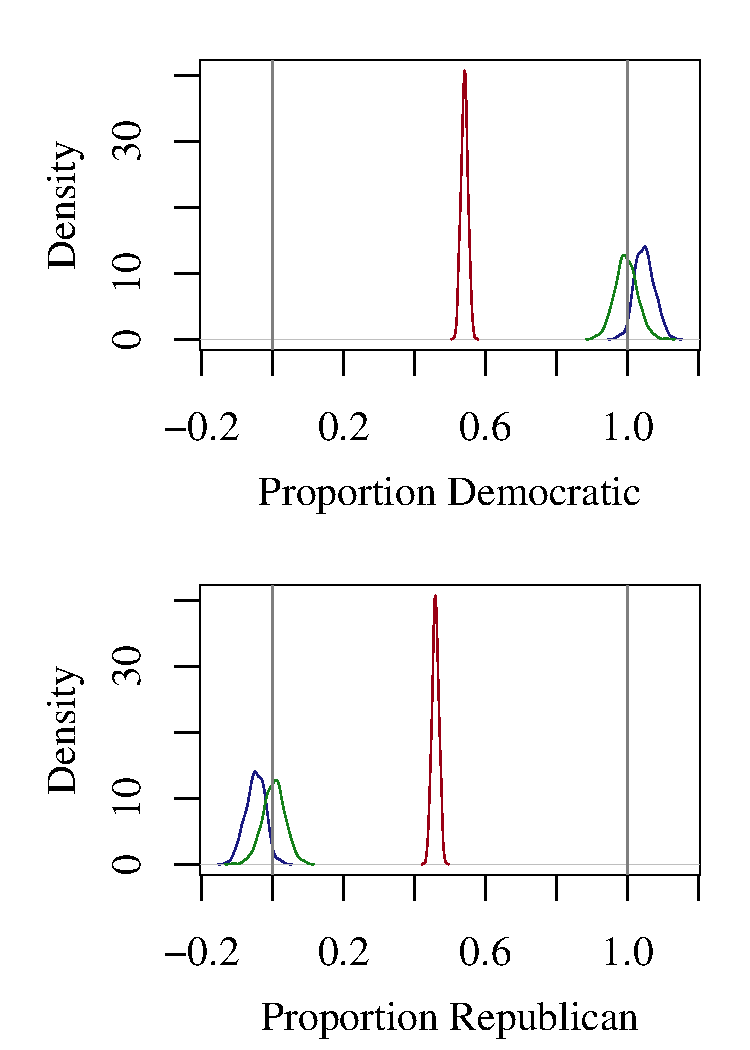
\includegraphics[height=3in]{eiBayesReg.pdf}
\end{center}
\caption{Density plots of ecological regression output.}
\label{f:er}
\end{figure}

%\item \begin{verbatim}
%ei.reg(cbind(dem, rep, non) ~ cbind(black, white, natam), 
%   data = senc)
%\end{verbatim}

%\begin{verbatim} 
%lambda.reg(out.reg, columns = c("dem", "rep")) 
%\end{verbatim}
%\item \texttt{density.plot} provides a graphical summary of \texttt{lambda} output:

\subsection*{Multinomial-Dirichlet (MD) model}

In the Multinomial-Dirichlet model proposed by \citet{RosJiaKin01},
the data is expressed as counts and a hierarchical Bayesian model is fit
using a Metropolis-within-Gibbs algorithm implemented in {\tt C}.
Level 1 models the observed column marginals as multinomial (and
independent across units); the choice of the multinomial corresponds
to sampling with replacement from the population.  Level 2 models the
unobserved row cell fractions as Dirichlet (and independent across
rows and units); Level 3 models the Dirichlet parameters as
i.i.d.\ Gamma.  More formally, without a covariate, the model is

\begin{eqnarray*}
(N_{\cdot 1i}, \dots, N_{\cdot Ci}) &\stackrel{\indep}{\sim}& {\rm
Multinomial}(N_i, \sum_{r=1}^R \beta_{r1i}X_{ri},\\ 
 & & \quad \dots, \sum_{r=1}^R \beta_{rCi}X_{ri}) \\
(\beta_{r1i}, \dots, \beta_{rCi}) &\stackrel{\indep}{\sim}& {\rm Dirichlet}(\alpha_{r1}, \dots, \alpha_{rC})\\
\alpha_{rc} &\stackrel{\rm i.i.d.}{\sim}& {\rm Gamma}(\lambda_1,\lambda_2) 
\end{eqnarray*}

With a unit-level covariate $Z_i$ in the second level, the model becomes
\begin{eqnarray*}
(N_{\cdot 1i}, \dots, N_{\cdot Ci}) &\stackrel{\indep}{\sim}& {\rm
Multinomial}(N_i, \sum_{r=1}^R \beta_{r1i}X_{ri},\\
 & & \quad \dots, \sum_{r=1}^R \beta_{rCi}X_{ri}) \\
(\beta_{r1i}, \dots, \beta_{rCi}) &\stackrel{\indep}{\sim}& {\rm
Dirichlet}(d_r e^{(\gamma_{rc} + \delta_{rc}Z_i)}, \dots, \\
& & \quad  d_r e^{(\gamma_{r(C-1)} +
\delta_{r(C-1)}Z_i)}, d_r ) \\
d_r &\stackrel{\rm i.i.d.}{\sim}& {\rm Gamma}(\lambda_1, \lambda_2)  
\end{eqnarray*}

In the model with a covariate, users have two options for the priors
on $\gamma_{rc}$ and $\delta_{rc}$ .  They may may assume an improper
uniform prior, as was
suggested by \citet{RosJiaKin01}, or they may specify normal priors
for each $\gamma_{rc}$ and $\delta_{rc}$ as follows:
\begin{eqnarray*}
\gamma_{rc} & \sim & {\rm N}(\mu_{\gamma_{rc}},
\sigma_{\gamma_{rc}}^2)\\
\delta_{rc} & \sim & {\rm N}(\mu_{\delta_{rc}}, \sigma_{\delta_{rc}}^2)   
\end{eqnarray*}
As \citet{Wakefield04} notes, the weak identification that
characterizes hierarchical models in the \acronym{ei} context is
likely to make the results sensitive to the choice of prior.  Users
should experiment with different assumptions about the prior
distribution of the upper-level parameters in order to gauge the
robustness of their inferences.

The parameterization of the prior on each $(\beta_{r1i}, \dots,
\beta_{rCi})$ implies that the following log-odds ratio of expected
fractions is linear with respect to the covariate $Z_i$:
\begin{displaymath}
\log\left( \frac{E(\beta_{rci})}{E(\beta_{rCi})} \right) = \gamma_{rc}
+ \delta_{rc} Z_i
\end{displaymath}


Conducting an analysis using the \acronym{md} model requires two steps.  First,
\command{tuneMD} calibrates the tuning parameters used for
Metropolis-Hastings sampling:
\begin{smallexample}
> tune.nocov <- tuneMD(cbind(dem, rep, non) 
+   ~ cbind(black, white, natam), data = senc, 
+   ntunes = 10, totaldraws = 100000)
\end{smallexample}
\noindent Second, \command{ei.MD.bayes} fits the model by calling
\texttt{C} code to generate \acronym{MCMC} draws:
\begin{smallexample}
> out.nocov <- ei.MD.bayes(cbind(dem, rep, non) 
+   ~ cbind(black, white, natam),
+   covariate = NULL, data = senc, 
+   tune.list = tune.nocov)
\end{smallexample}
The output of this function can be returned as \code{mcmc} objects
or arrays; in the former case, the standard diagnostic tools in
\pkg{coda} \citep{PlummerEtal06} can be applied directly.   The \acronym{md} implementation includes \command{lambda} and \command{density.plot}
functions, usage for which is analogous to ecological regression:
\begin{smallexample}
> lmd <- lambda.MD(out.nocov, 
+   columns = c("dem", "rep"))
> density.plot(lmd)
\end{smallexample}
If the precinct-level parameters are returned or saved,
\command{cover.plot} plots the central credible intervals for each
precinct.  The segments represent the 95\% central credible intervals
and their medians for each unit (the true value for each precinct is
the red dot, not included in the standard \command{cover.plot}).
\begin{smallexample}
> cover.plot(out.nocov, row = "white", 
+   column = "dem")
# add true values to plot
> points(senc$white/senc$total, 
+   senc$whdem/senc$white)
\end{smallexample}
\begin{figure}[h]
\begin{center}
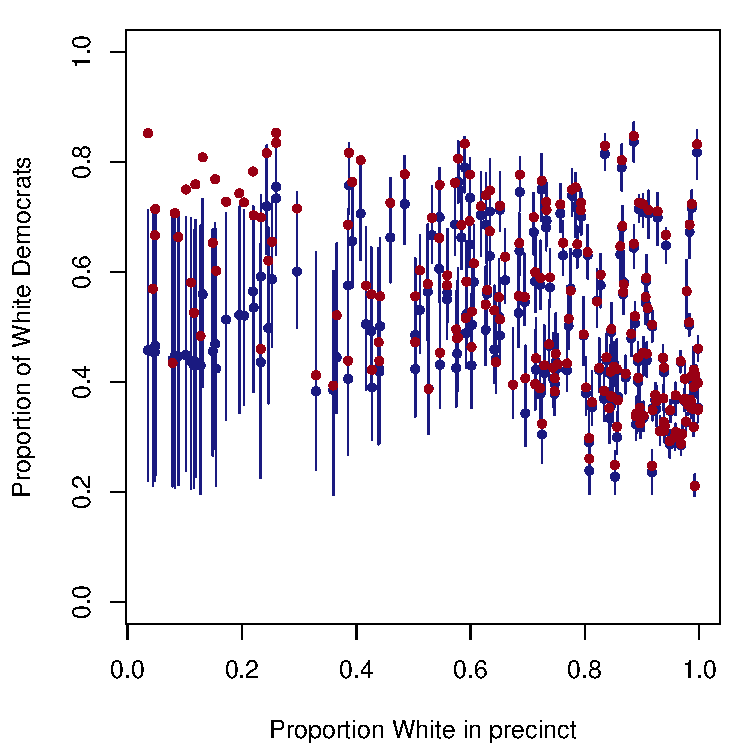
\includegraphics[width=3in]{coversmall.pdf}
\end{center}
\caption{Coverage plot for {\sc md} model output.}
\label{f:md}
\end{figure}
 
\section*{Data Management}

In the \acronym{md} model, reasonable-sized problems produce unreasonable
amounts of data.  For example, a model for voting in Ohio includes
11000 precincts, 3 racial groups, and 4 parties.  Implementing 1000
iterations yields about 130 million parameter draws.  These draws
occupy about 1GB of \acronym{RAM}, and this is almost certainly not enough
iterations.  We provide a few options to users in order to make this
model tractable for large \acronym{ei} problems. 

The unit-level parameters present the most significant data management
problem.  Rather than storing unit-level parameters in the workspace, users can
save each chain as a \code{.tar.gz} file on disk using the option
\code{ei.MD.bayes(..., ret.beta = "s")}, or discard the unit-level
draws entirely using \code{ei.MD.bayes(..., ret.beta = "d")}.  To
reconstruct the chains, users can select the row marginals, column
marginals, and units of interest, without reconstructing the entire
matrix of unit-level draws:   
\begin{smallexample}
> read.betas(rows = c("black", "white"), 
+   columns = "dem", units = 1:150, 
+   dir = getwd())
\end{smallexample}
If users are interested in some function of the unit-level parameters,
the implementation of the \acronym{md} model allows them to define a
function in \R{} that will be called from within the {\tt C}
sampling algorithm, in which case the unit-level parameters need not
be saved for post-processing.

\section*{Acknowledgments}

\pkg{eiPack} was developed with the support of the Institute for
Quantitative Social Science at Harvard University.  Thanks to John
Fox, Gary King, Kevin Quinn, D. James Greiner, and an anonymous
referee for suggestions and Matt Cox and Bob Kinney for technical
advice.  For further information, see
\url{http://www.people.fas.harvard.edu/~olau/software/eiPack.html}.


\begin{thebibliography}{9}
\expandafter\ifx\csname natexlab\endcsname\relax\def\natexlab#1{#1}\fi
\expandafter\ifx\csname url\endcsname\relax
  \def\url#1{{\tt #1}}\fi

\bibitem[Cho and Yoon(2001)]{Cho01}
W.~T. Cho and A.~H. Yoon.
\newblock Strange bedfellows: Politics, courts and statistics: Statistical
  expert testimony in voting rights cases.
\newblock {\em Cornell Journal of Law and Public Policy}, 10:\penalty0
  237--264, 2001.

\bibitem[Duncan and Davis(1953)]{DunDav53}
O.~D. Duncan and B.~Davis.
\newblock An alternative to ecological correlation.
\newblock {\em American Sociological Review}, 18:\penalty0 665--666, 1953.

\bibitem[Goodman(1953)]{Goodman53}
L.~Goodman.
\newblock Ecological regressions and the behavior of individuals.
\newblock {\em American Sociological Review}, 18:\penalty0 663--664, 1953.

\bibitem[Grofman(2000)]{Grofman00}
B.~Grofman.
\newblock A primer on racial bloc voting analysis.
\newblock In N.~Persily, editor, {\em The Real {Y}2{K} Problem: Census 2000
  Data and Redistricting Technology}. Brennan Center for Justice, New York,
  2000.

\bibitem[Imai and Lu(2005)]{eco}
K.~Imai and Y.~Lu.
\newblock {\em eco: R Package for Fitting Bayesian Models of Ecological
  Inference in 2x2 Tables}, 2005.
\newblock URL \url{http://imai.princeton.edu/research/eco.html}.

\bibitem[Martin and Quinn(2006)]{MartinQuinn06}
A.~D. Martin and K.~M. Quinn.
\newblock Applied {B}ayesian inference in {R} using {MCMC}pack.
\newblock {\em R News}, 6:\penalty0 2--7, 2006.

\bibitem[Plummer et~al.(2006)Plummer, Best, Cowles, and Vines]{PlummerEtal06}
M.~Plummer, N.~Best, K.~Cowles, and K.~Vines.
\newblock {CODA}: Convergence diagnostics and output analysis for {MCMC}.
\newblock {\em R News}, 6:\penalty0 7--11, 2006.

\bibitem[Rosen et~al.(2001)Rosen, Jiang, King, and Tanner]{RosJiaKin01}
O.~Rosen, W.~Jiang, G.~King, and M.~A. Tanner.
\newblock Bayesian and frequentist inference for ecological inference: The ${R}
  \times {C}$ case.
\newblock {\em Statistica Neerlandica}, 55\penalty0 (2):\penalty0 134--156,
  2001.

\bibitem[Wakefield(2004)]{Wakefield04}
J.~Wakefield.
\newblock Ecological inference for 2 $\times$ 2 tables (with discussion).
\newblock {\em Journal of the Royal Statistical Society}, 167:\penalty0
  385--445, 2004.

\end{thebibliography}





\begin{flushleft}
\address{Olivia Lau}\\
\email{olau@fas.harvard.edu}\\
\emph{Ryan T. Moore}\\
\email{rtmoore@fas.harvard.edu}\\
\emph{Michael Kellermann}\\
\email{kellerm@fas.harvard.edu}\\
\address{Institute for Quantitative Social Science\\
Harvard University, Cambridge, MA}
\end{flushleft}

